\chapter{基于BLE Mesh的智能家居平台功能设计}

\section{架构设计}
本项目主要分为三个部分:BLE Mesh节点,网关端及移动端(如图~\ref{fig:arch_basic})。

BLE Mesh节点主要实现传感器、继电器、灯泡等设备的接入,并且节点间可自动建立BLE协议下的Mesh网络,使得用户即使不使用网关也能用移动端软件连接至Mesh网络控制所有节点。

网关端主要实现设备层与管理应用层的连接。采用插件化的方案,使得有能力的爱好者或其他智能设备厂商,可以自己根据本项目简单的API来制作插件接入本平台;也便于接入到其他的管理平台,例如Apple HomeKit、Google Home等,让用户不需要下载其他程序就能管理网关下的所有设备。

移动端主要实现控制Mesh网络或网关下的设备、添加自动化的功能。
\begin{figure}[H]
    \centering
    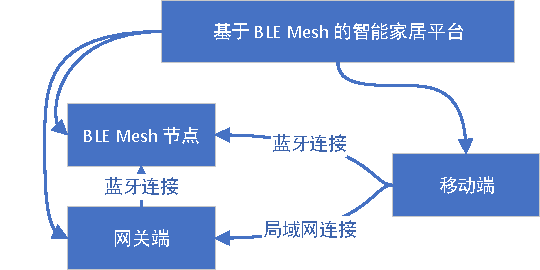
\includegraphics{arch_basic.pdf}
    \caption{基于BLE Mesh的智能家居平台基本架构图}
    \label{fig:arch_basic}
\end{figure}

\section{BLE Mesh节点}
\label{design:blemeshnode}
BLE Mesh节点不同于一般智能家居设备,它们之间通过另一个BLE Mesh分发节点或手机分发配置后构成网状网络,之后所有数据就可通过其他节点转发至目标设备(如图~\ref{fig:arch_mesh})。

每个节点均可接入多个模块,例如继电器、开关、传感器等。不需要每个模块都单独配一套蓝牙通讯装置,节约了成本也节约了频段资源。

网关或移动端设备也可以通过任一节点代理入Mesh网络,之后便可以访问所有的节点及其连接的模块。
\begin{figure}[H]
    \centering
    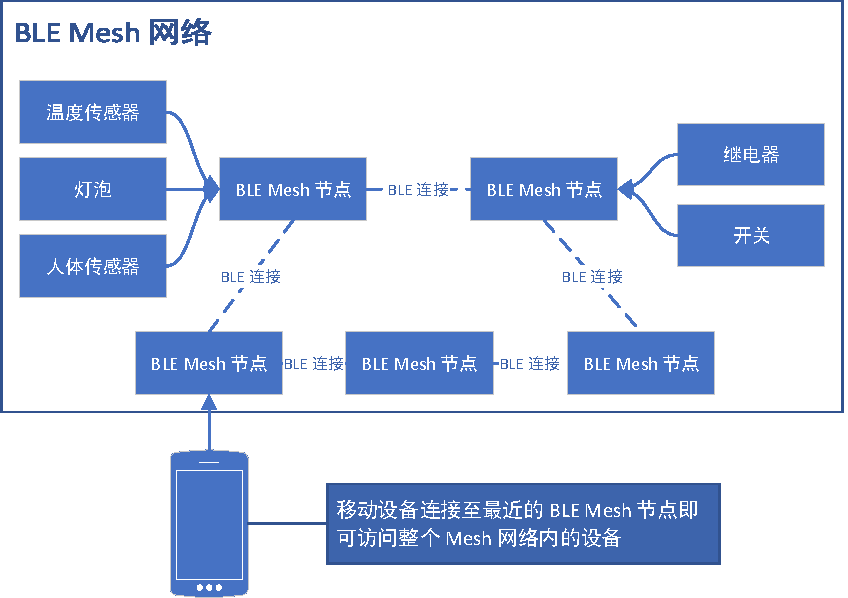
\includegraphics{arch_mesh.pdf}
    \caption{基于BLE Mesh的智能家居平台BLE Mesh网络架构图}
    \label{fig:arch_mesh}
\end{figure}

\section{网关端}
网关端实现了设备层与管理应用层的连接,即将不同的智能设备(如~\ref{design:blemeshnode}~章所提到的BLE Mesh节点等)与不同的管理平台(如~\ref{design:mobile}~章所提到的基于BLE Mesh的智能家居平台移动端、Apple HomeKit等)相连接。

网关端还创新性地采用了插件化的方案(如图~\ref{fig:arch_gateway}),使得爱好者或智能家居厂商可自行按照网关端插件API编写对应插件,让家中所有的智能设备最终能在一个平台上进行管理。目前本项目已开发的插件有BLE Mesh插件(用于连接BLE Mesh节点)、本项目移动端所使用的WebSocket插件(将设备以WebSocket的方式暴露到内网便于移动端连接)以及Apple HomeKit插件(将设备以符合Apple HomeKit方式暴露到内网便于苹果设备上的“家庭”应用连接)。
\begin{figure}[H]
    \centering
    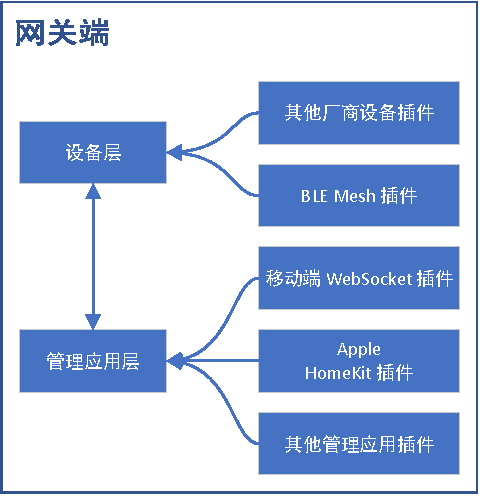
\includegraphics{arch_gateway.pdf}
    \caption{基于BLE Mesh的智能家居平台网关端架构图}
    \label{fig:arch_gateway}
\end{figure}

\section{移动端}
\label{design:mobile}
移动端包含了UI层、设备层及自动化层(如图~\ref{fig:arch_mobile})。UI层支持用户查看所有设备的状态、控制所有设备及添加自动化流程。设备层支持通过单个BLE Mesh节点代理入网的方式及通过连接至网关端WebSocket插件的方式访问整个智能家居网络。而自动化层支持用户将只包含网关设备的自动化流程提交到网关。
\begin{figure}[H]
    \centering
    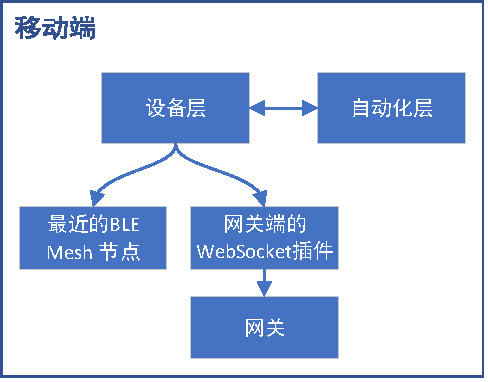
\includegraphics{arch_mobile.pdf}
    \caption{基于BLE Mesh的智能家居平台移动端架构图}
    \label{fig:arch_mobile}
\end{figure}
